\apendice{Especificación de diseño}\label{anex:C}

\section{Introducción}
En este apartado recogen las causas por las que se han adoptado las soluciones de diseño del software desarrollado, divididas diseño de datos, arquitectónico y diseño de la interfaz de usuario.

\section{Diseño de datos}\label{sec:C_2}
Las entidades con las que se trabaja en el proyecto son clases de \textit{Java}. Si en un futuro se trabajase con una base de datos se podrían convertir las entidades de ésta a las clases \textit{Java} que se utilizan actualmente sin mayor problema.

En el paquete \textit{datamodel} podemos encontrar las clases más importantes en relación a los datos:
\begin{itemize}
	\item \ruta{Repository}. Sirve como definición de los datos que se obtienen de un repositorio. Estos datos son:
	\begin{itemize}
		\item URL, nombre e ID del proyecto
		\item Métricas internas (\ruta{RepositoryInternalMetrics}). Representan los valores de los que se obtienen las métricas externas y que interesan para satisfacer los requisitos funcionales de la aplicación. Esta clase contiene toda la información de un repositorio necesaria para calcular las métricas, que es la fecha de medición, el número total de issues, el número total de commits, el número de issues cerradas, una colección de días que se tardan en cerrar las issues, otra colección con las fechas de los commits, el tiempo de vida del proyecto, una colección de los \textit{jobs} del proyecto y una colección de las \textit{releases} del proyecto.\\
		Cabe indicar que se define el método \textit{equals} a partir de la fecha de medición.
		\item Resultados de las métricas (\ruta{MetricsResults}). Al añadir un repositorio estos se calcularán y quedarán almacenados en una instancia de esta clase.
		\item Evaluación del proyecto (\textit{projectEvaluation}). En esta clase se evalúan las diferentes métricas en función de sus umbrales y se almacena el porcentaje de métricas evaluadas como `buenas' cada vez que se calcule alguna de ellas.
		\item Cabe indicar que se ha definido la igualdad de los repositorios en base a su URL, ID y nombre.
	\item \ruta{User}. Sirve para almacenar información que se obtiene de las forjas de repositorios acerca del usuario que ha iniciado sesión. Se almacenan la ID de usuario, la URL del avatar, el email, el nombre y el nombre de usuario.
	\end{itemize}
	\item Se han implementado clases personalizadas para envolver a las clases relacionadas con los \textit{jobs} del proyecto y una colección de las \textit{releases} devueltas por las librerías de integración con las forjas de repositorios. Esto ha sido necesario ya que las clases obtenidas por medio de las librerías de conexión no son serializables y en la aplicación necesitamos serializar los resultados de las métricas para poder exportarlos e importarlos.\\
	Las clases generadas son: \textit{CustomGithubApiJob}, \textit{CustomGithubApiRelease}, \textit{CustomGitlbApiJob} y \textit{CustomGitlabApiRelease}.\\
	Hay que indicar que en estas clases se han de almacenar como variables aquellas que se tengan que usar para los cálculos de las métricas, por ejemplo el nombre de los \textit{jobs} con \textit{this.job = job.getName()} para el cálculo de la métrica IC3.
\end{itemize}

El diagrama de clases de este paquete se puede ver en la figura \ref{fig:AnexC_Datamodel-ClassDiagram}

\begin{figure}[!h]
	\centering
	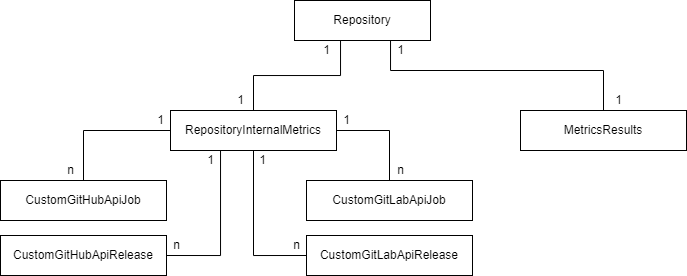
\includegraphics[width=1\textwidth]{AnexC_Datamodel-ClassDiagram}
	\caption{Paquete \textit{datamodel}}\label{fig:AnexC_Datamodel-ClassDiagram}
\end{figure}
\FloatBarrier
	
\section{Diseño arquitectónico}
A continuación se describe la estructura de paquetes del proyecto y las clases que contienen.

\subsection{Paquete \textit{repositorydatasource}}
El paquete define el \textit{framework} de conexión a una forja de repositorios e implementa la conexión tanto \textit{GitHub} como a \textit{GitLab}.

\imagen{AnexC_RepositoryDataSource}{Paquete \textit{repositorydatasource}}

Para crear un \textit{Repositorydatasource} con acceso a otra forja solo se tiene que implementar las dos interfaces, sin necesidad de hacer más cambios en el código, como se puede ver en la imagen la implementación para GitHub y GitLab es equivalente.

\subsection{Paquete metricsengine}
En este paquete se define el \textit{framework} de medición y sigue el diseño descrito en \textit{Soporte de Métricas con Independencia del Lenguaje para la Inferencia de Refactorizaciones} \cite{marticorena_sanchez_soporte_2005}, con unos pequeños cambios:

\begin{itemize}
	\tightlist
	\item Se ha aplicado a las métricas concretas el patrón \textit{\textbf{Singleton}} \footnote{\url{https://refactoring.guru/design-patterns/singleton}}, que obliga a que solo haya una única instancia de cada métrica. Además, se ha aplicado el patrón \textit{\textbf{Método fábrica}} \footnote{\url{https://refactoring.guru/design-patterns/factory-method}} tal y como se muestra en la Fig. \ref{fig:M3_CambiosFrameworkMedicion1}, de forma que \textit{MetricConfiguration} no esté asociada con la métrica en sí, sino con una forma de obtenerla.\\
	El objetivo de trabajar de esta manera es facilitar la persistencia de un perfil de métricas. Las métricas se podrían ver como clases estáticas, no varían en tiempo de ejecución y solo debería haber una instancia de cada una de ellas. Por ello, al importar o exportar un perfil de métricas con su conjunto de configuraciones de métricas, estas configuraciones no deberían asociarse a la métrica, sino a la forma de acceder a la única instancia de esa métrica. 
	\item Se trabaja con los métodos \textit{evaluate} y \textit{getEvaluationFunction} en la interfaz \textit{IMetric}, ver Fig. \ref{fig:M3_CambiosFrameworkMedicion2}, para obtener los valores de las mismas, siendo estos métodos un añadido que se realizó al \textit{framework} de medición original.\\
	Esto permite interpretar y evaluar los valores medidos sobre los valores límite de la métrica o configuración de métrica deduciéndose si su valor es bueno o no según el perfil de evaluación.\\
	 Por ejemplo, puede que para unas métricas un valor aceptable esté comprendido entre el valor límite superior y el valor límite inferior; y para otras un valor aceptable es aquel que supere el límite inferior.\\
	\textit{EvaluationFunction} es una interfaz funcional \footnote{Enlaces a la documentación: \url{https://docs.oracle.com/javase/8/docs/api/java/lang/FunctionalInterface.html} --- \url{https://docs.oracle.com/javase/8/docs/api/java/util/function/package-summary.html}} 
	de tipo `\textit{función}': recibe uno o más parámetros y devuelve un resultado. Este tipo de interfaces son posibles a partir de la versión 1.8 de \textit{Java}.\\
	Esto permite definir los tipos de los parámetros y de retorno de una función que se puede almacenar en una variable. De este modo se puede almacenar en una variable la forma en la que se puede evaluar la métrica.
\end{itemize}

\imagen{M3_CambiosFrameworkMedicion1}{Patrones ``\textit{singleton}'' y ``método fábrica'' sobre el \textit{framework} de medición}

\imagen{M3_CambiosFrameworkMedicion2}{Añadido al \textit{framework} de medición la evaluación de métricas}

\subsection{Paquete \textit{gui}}
En este paquete se define toda la interfaz gráfica.


\subsection{Paquete \textit{exceptions}}
En este paquete se encuentran las excepciones de la aplicación, además se trabaja con códigos de error y mensajes para poder ser identificados y comprendidos en el \textit{logger} fácilmente. Se ha creado un diseño en el que, para definir nuevas excepciones, se puede extender de \textit{ApplicationException}, copiar y adaptar los constructores y modificar con \textit{@Override} el método \textit{generateMessage()} con los mensajes personalizados en un \textit{switch} para cada código de error:

\begin{figure}[!h]
	\centering
	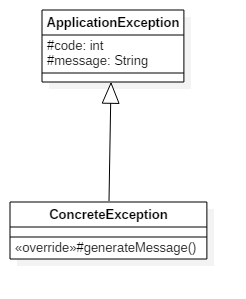
\includegraphics[width=0.5\textwidth]{AnexC_Exceptions}
	\caption{Paquete \textit{exceptions}}\label{fig:AnexC_Exceptions}
\end{figure}
\FloatBarrier

Trabajando con este diseño se han podido implementar excepciones para las nuevas métricas.

\subsection{Paquete \textit{datamodel}}
El paquete \textit{datamodel} contiene las diferentes clases que se han descrito anteriormente en la sección \ref{sec:C_2}. Si en un futuro se integraran nuevas forjas de repositorios puede que sea necesario añadir nuevas clases de envoltura para serializar los valores que obtengamos como se ha visto anteriormente.

\subsection{Paquete \textit{app}}
Contiene las clases que sirven de conexión entre la interfaz de usuario y la lógica de la aplicación.

\begin{figure}[!h]
	\centering
	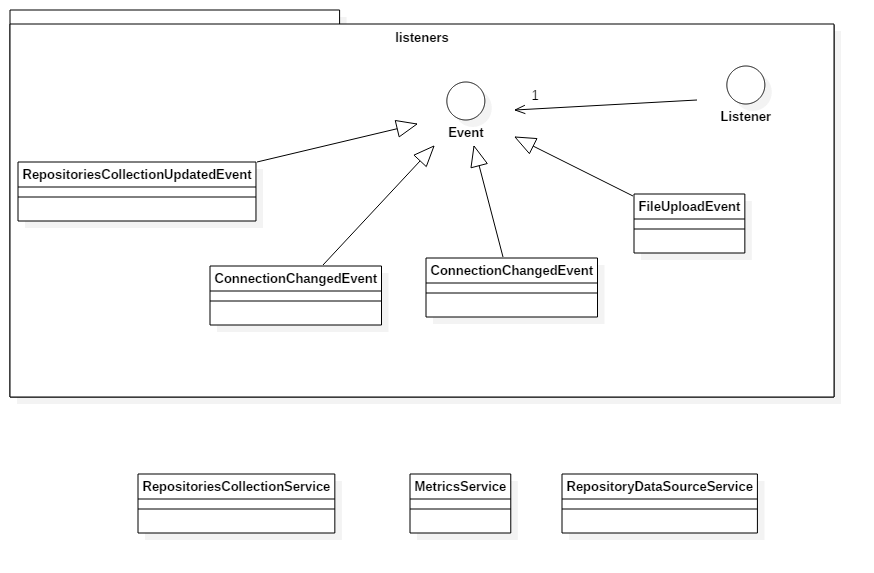
\includegraphics[width=1\textwidth]{AnexC_app}
	\caption{Paquete \textit{app}}\label{fig:AnexC_app}
\end{figure}
\FloatBarrier

Las clases que encontramos en este paquete son:
\begin{description}
	\item[\textit{MetricsService}] Define una fachada de conexión entre el motor de métricas y el resto de componentes.
	\item[\textit{RepositoriesCollectionService}] Se encarga de almacenar los repositorios en una colección
	\item[\textit{RepositoriesCollectionService}] Define una fachada entre la fuente de datos (\textit{repositorydatasource}) y el resto de componentes.
\end{description}

\subsubsection{Paquete \textit{app.listeners}}
En este paquete trabajamos con el patrón observador. Se definen la interfaz \textit{Listener} y la interfaz \textit{Event} y se implementan algunos eventos como el de conexión a una forja o el de subida de un archivo para realizar diferentes acciones cuando se den dichos eventos.\\ 
La interfaz \textit{Event} sirve para implementar eventos a partir de ella, estos eventos normalmente tienen información relativa al suceso que ocurre. Por ejemplo, \textit{CurrentMetricProfileChangedEvent} contiene información sobre un cambio de perfil de métricas: el viejo perfil y el nuevo. La interfaz \textit{Listener} define una función a la que se le pasa un evento y sirve como interfaz funcional para ejecutar una acción (función lambda) que recibe por parámetro el evento.
